\chapter{Introduction}
\section{Motivation and goals}
Data compression plays a key role in remote sensing, specially in hazardous environments, where computing power and data links are limited. Two examples of these environments are deep space and offshore. In addition, some technologies used to capture data are proprietary and the data structure may not be optimal for general purpose compressors such as GZIP.

This thesis is part of two strategic projects of DAPCOM Data Services, a spin-off company of the \acrshort{upc} and \acrshort{ub}. The first project is intended to compress \acrfull{rf} data, mainly from \acrshort{sdr} devices; the second one is focused on compressing the water column information contained in the KMALL format, a new data structure from the multinational Kongsberg Maritime.

We aim to develop two \acrshort{fapec} stages to perform better, in terms of compression ratio and speed, than already existing algorithms. Specifically, we will compare the first stage with \acrshort{flac}, a well-known audio encoder, and GZIP. The second stage will be only compared with GZIP, as we have not been able to find any specific compressor for such format. Additionally, we also want to propose a universal metric to reliably quantify the performance of new stages in terms of information redundancy.

\section{Thesis outline and organization}
This thesis starts in chapter \ref{ch:entropy_coding} with a theoretical approach to information theory. There, we describe some basic concepts which will be used later, such as differential entropy or Golomb coding.

In chapter \ref{ch:fapec} we describe the key aspects of the \acrshort{fapec} data compression framework and the current features and stages. Then, in chapter \ref{ch:new_stages} we state the general requirements and specifications for the new stages. In this chapter we also propose some metrics to evaluate preprocessing stages.

The next two chapters correspond to the two preprocessing stages we have developed. The outline for both chapters \ref{ch:wave_preproc} and \ref{ch:kmall_preproc} is almost the same: first, we introduce the data format. Then, we propose an algorithm, and finally, we evaluate it using the metrics from chapter \ref{ch:new_stages}.

Finally, the last chapter consists in concluding the thesis and describing some possible future lines to work with.

The \LaTeX{} source code and the Python scripts used to evaluate the stages can be found in the GitHub repository: \url{https://github.com/aniolm9/bsc-thesis-fapec}.

\section{State of the art}
Compressing \acrshort{rf} data using \acrshort{flac} is not new. For instance, there is a paper \parencite{IQFlac} where \acrshort{flac} is applied on \acrshort{iq} data. This paper together with reports from some DAPCOM clients may serve as a basis to develop a new algorithm.

On the other hand, the KMALL stage has been mainly based on the stage that DAPCOM developed in 2019 for the old water column data structure \parencite{Portell2019}. As the KMALL format was released in 2019, very few literature exists, but we have found a paper \parencite{MBESComp} where the authors propose a modification of Huffman coding to compress \acrshort{mwc} data in older formats. Although the entropy analysis they do is of much interest, the proposed algorithm is mostly based on plain entropy coding, so it is not very useful in our case.

Finally, as regards to the universal metric to evaluate stages, we have found some interesting papers \parencite{negentropy} \parencite{HYVARINEN2000411} where the authors explore ways to measure the distance of some data to gaussianity.

\section{Project planning and costs}
\subsection{Gantt diagram}
\begin{figure}[h!]
	\begin{center}
		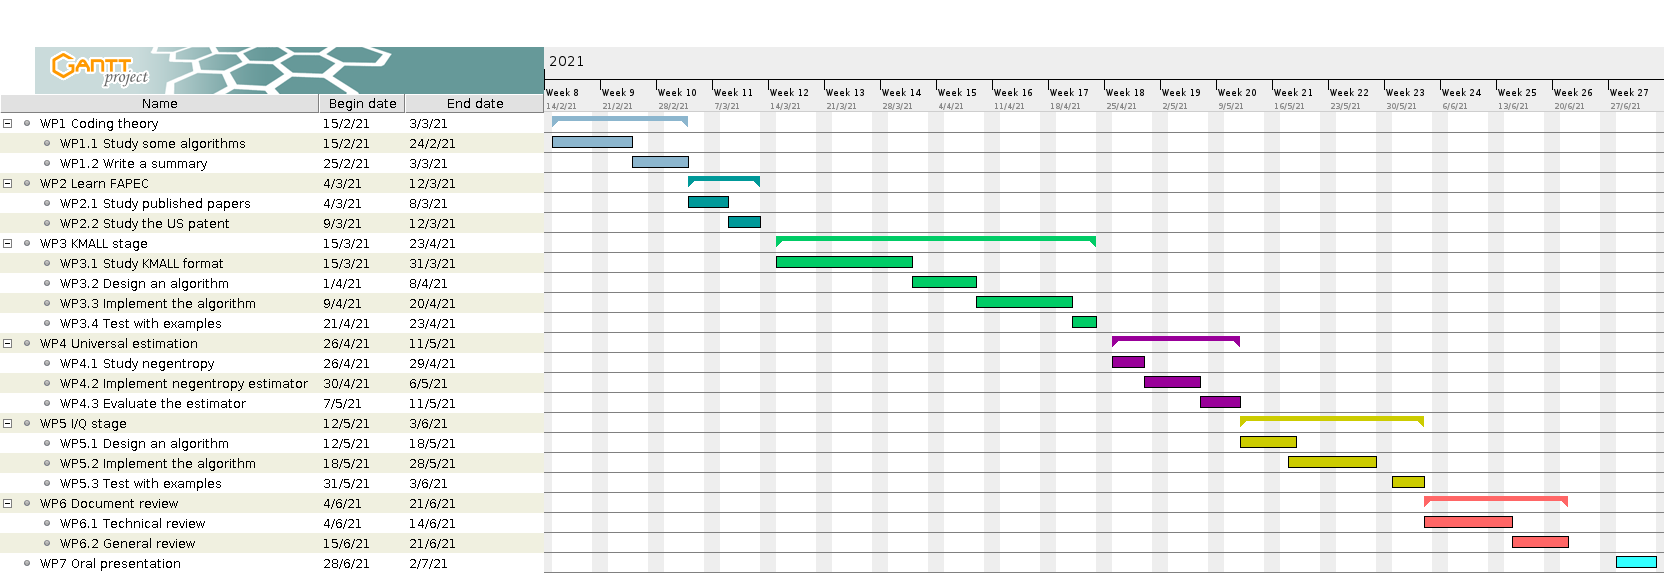
\includegraphics[scale=0.255]{images/gantt.png}
	\end{center}
	\caption{Project Gantt diagram.}
	\label{fig:gantt}
\end{figure}

\subsection{Budget and costs}
This thesis consists in the design, implementation and evaluation of two stages which will be included in a bigger framework, \acrshort{fapec}. In this situation, a straightforward financial study is not possible and going further is clearly out of scope.

However, this thesis has been developed within a cooperation agreement between the \acrfull{upc} and DAPCOM Data Services, with a cost of 3816€.
